\documentclass{article}
\usepackage[utf8]{inputenc}
\usepackage[margin=1.2in]{geometry}
\usepackage{graphicx}
\usepackage{mdwlist}


\def\answer#1{
    \vspace*{0.5em}\\
    \noindent\fbox{%
    \parbox{\textwidth}{%
		#1
    }%
}
}

\newcommand{\mycoursenum}{15-440/15-640}
\newcommand{\myhwnum}{1}
\newcommand{\myname}{}   % put your name here
\newcommand{\myandrew}{}  % put your andrewID here

\newif\ifprint
\printtrue  % change to printfalse after adding your name and andrewID

\def\changemargin#1#2{\list{}{\rightmargin#2\leftmargin#1}\item[]}
\let\endchangemargin=\endlist 

\begin{document}
\medskip
\thispagestyle{plain}
\begin{center}
{\Large \mycoursenum: Homework \myhwnum}\\
Due: September 27, 2016 10:30am \\
\medskip
\ifprint
Name: \rule{0.5\textwidth}{.4pt} \\
Andrew ID: \rule{0.45\textwidth}{.4pt} \\
\else
Name: \myname \\
Andrew ID: \myandrew \\
\fi
\end{center}

\begin{enumerate}

\item Alice wants to send files to Bob over the Internet at the fastest possible speed. To find the best network setting among those available to her, she transfers a 1000 KByte file over three different network settings. Calculate the total time taken to transfer this file in each of the following scenarios and help Alice decide which of those is the network setting she should use.\\
For each of the following three scenarios calculate the total time taken to transfer the file assuming that the packet size is 1KByte, the RTT is 100ms, and that an initial 2*RTT of handshaking is performed before the actual data is sent.
    \begin{enumerate}
    \item Data packets are sent continuously on a 1.5Mbps bandwidth link \textbf{[5 points]}
    \item After sending each data packet, there is a wait time of 1 RTT before sending the next packet. The link bandwidth is 1.5 Mbps. \textbf{[5 points]}
    \item Up to 20 packets can be sent per RTT, and the bandwidth is infinite, i.e., the transmit time is zero \textbf{[5 points]}   
    \end{enumerate}

\item Consider the following network topology, with hosts A and B connected through router R: 

\vspace{0.25in}
\begin{center}
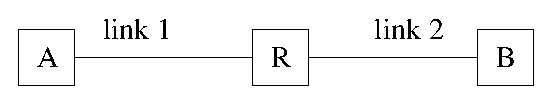
\includegraphics[width=.4\textwidth]{sh_flow_control.eps}
\end{center}
\vspace{0.25in}

Router R operates in store-and-forward mode. Links 1 and 2 are both one megabit per second links with 10ms one-way latency.

    \begin{enumerate}
    \item How long does it take to send a 1000 bit packet from A to B? \textbf{[5 points]}
    \item Recall that in Stop-and-Wait flow control mechanism, the sender sends a packet and then ‘stops and waits’ for an ACK before sending the next packet. Using stop-and-wait flow control, how long does it take for A to send a 100,000 bit file to B?  Assume that the data packets are 1000 bits long. \textbf{[5 points]}
    \item What should be the minimum appropriate window size (the number of packets sent by the sender before waiting for an ACK) to utilize the full link bandwidth? \textbf{[5 points]} 
    \item Generalize the appropriate window size W from part (c), for an arbitrary bandwidth B, a packet size N and an RTT R. \textbf{[5 points]}
    \end{enumerate}

\newpage
\item Answer the following with respect to Remote Procedure Calls \textbf{[8 points]}
    \begin{enumerate}
    \item Describe two ways in which RPC calls differ from local procedure calls
    
    \item Describe how you could help deal with each of the differences listed in part (a).
    \end{enumerate}
    
    
\item
In the following situations, describe which RPC semantic is the most suitable (at-most-once or at-least-once), and why.\textbf{[8 points]}
    \begin{enumerate}
    \item Saving a file in a distributed file system
    \item Buying a laptop online
    \item Checking the price of a stock
    \item Uploading a blog post

    \end{enumerate}

\item
There is a classical problem in concurrency known as the “Dining Philosophers.” The problem is as follows: There are 5 philosophers sitting around a circular dining table. Each philosopher has a bowl of rice in front of him, and there is a single chopstick in between each two philosophers. Each philosopher alternates between thinking and eating. A philosopher needs a pair (i.e. fork to their left AND right) of chopsticks in order to eat. When the philosopher is done eating and goes back to thinking, he will put down his chopsticks. 

    \begin{enumerate}
    \item Given that this is an example of a concurrent system with a need for synchronization, a solution should aim for i) correctness, ii) efficiency, and iii) fairness. Describe what each goal means in the context of the Dining Philosophers problem. \textbf{[3 points]}
    
    \suspend{enumerate}
    
    \texttt{Step 1:} think until the left chopstick is available; when it is, pick up; \\
    \texttt{Step 2:} think until the right chopstick is available; when it is, pick up;\\
    \texttt{Step 3:} when both chopsticks are held, eat for a fixed amount of time;\\
    \texttt{Step 4:} then, put the right chopstick down;\\
    \texttt{Step 5:} then, put the left chopstick down;\\
    \texttt{Step 6:} repeat from the beginning.\\
    
    \resume{enumerate}
    \item Does this solution address the desirable properties of concurrent systems listed above? If not, which one is violated and give an example of when it is violated? \textbf{[6 points]}

    \item Assume that we change the solution outlined in part (b) above such that there is an additional waiter who allows only 4 philosophers at the table at any given time. The waiter will only allow another philosopher to join once there are \textless 4 philosophers at the table. Is there a desirable property of concurrent systems that is still violated? If so, give an example of when it is violated. \textbf{[6 points]}
    
    \end{enumerate}


\item
After forgetting your AFS password, you decide to create your own distributed file system. personal distributed file system to synchronize your files between your different devices. 
    \begin{enumerate}
    \item You want to design your distributed file system for personal use so you can synchronize your files between your different devices. Of the three main tradeoffs of distributed file systems: consistency, performance, and scalability, which would you optimize? Describe one way you would optimize this goal. \textbf{[5 points]}

    \item In order to work on group projects, you decide to open up your distributed file system to your group members. To ensure your work is not lost, you wish to replicate data in other servers. However, you have trouble deciding how data replication should be handled. Name one benefit of using AFS’s data replication method and one benefit of using Coda’s data replication method. \textbf{[6 points]}
    \end{enumerate}

\newpage
\item Processes 1, 2, 3 are using a logical clock to keep a consistent time. The horizontal arrow represents physical time and the crossing arrow represents a message being passed. Each point on the horizontal lines is an event.


\begin{center}
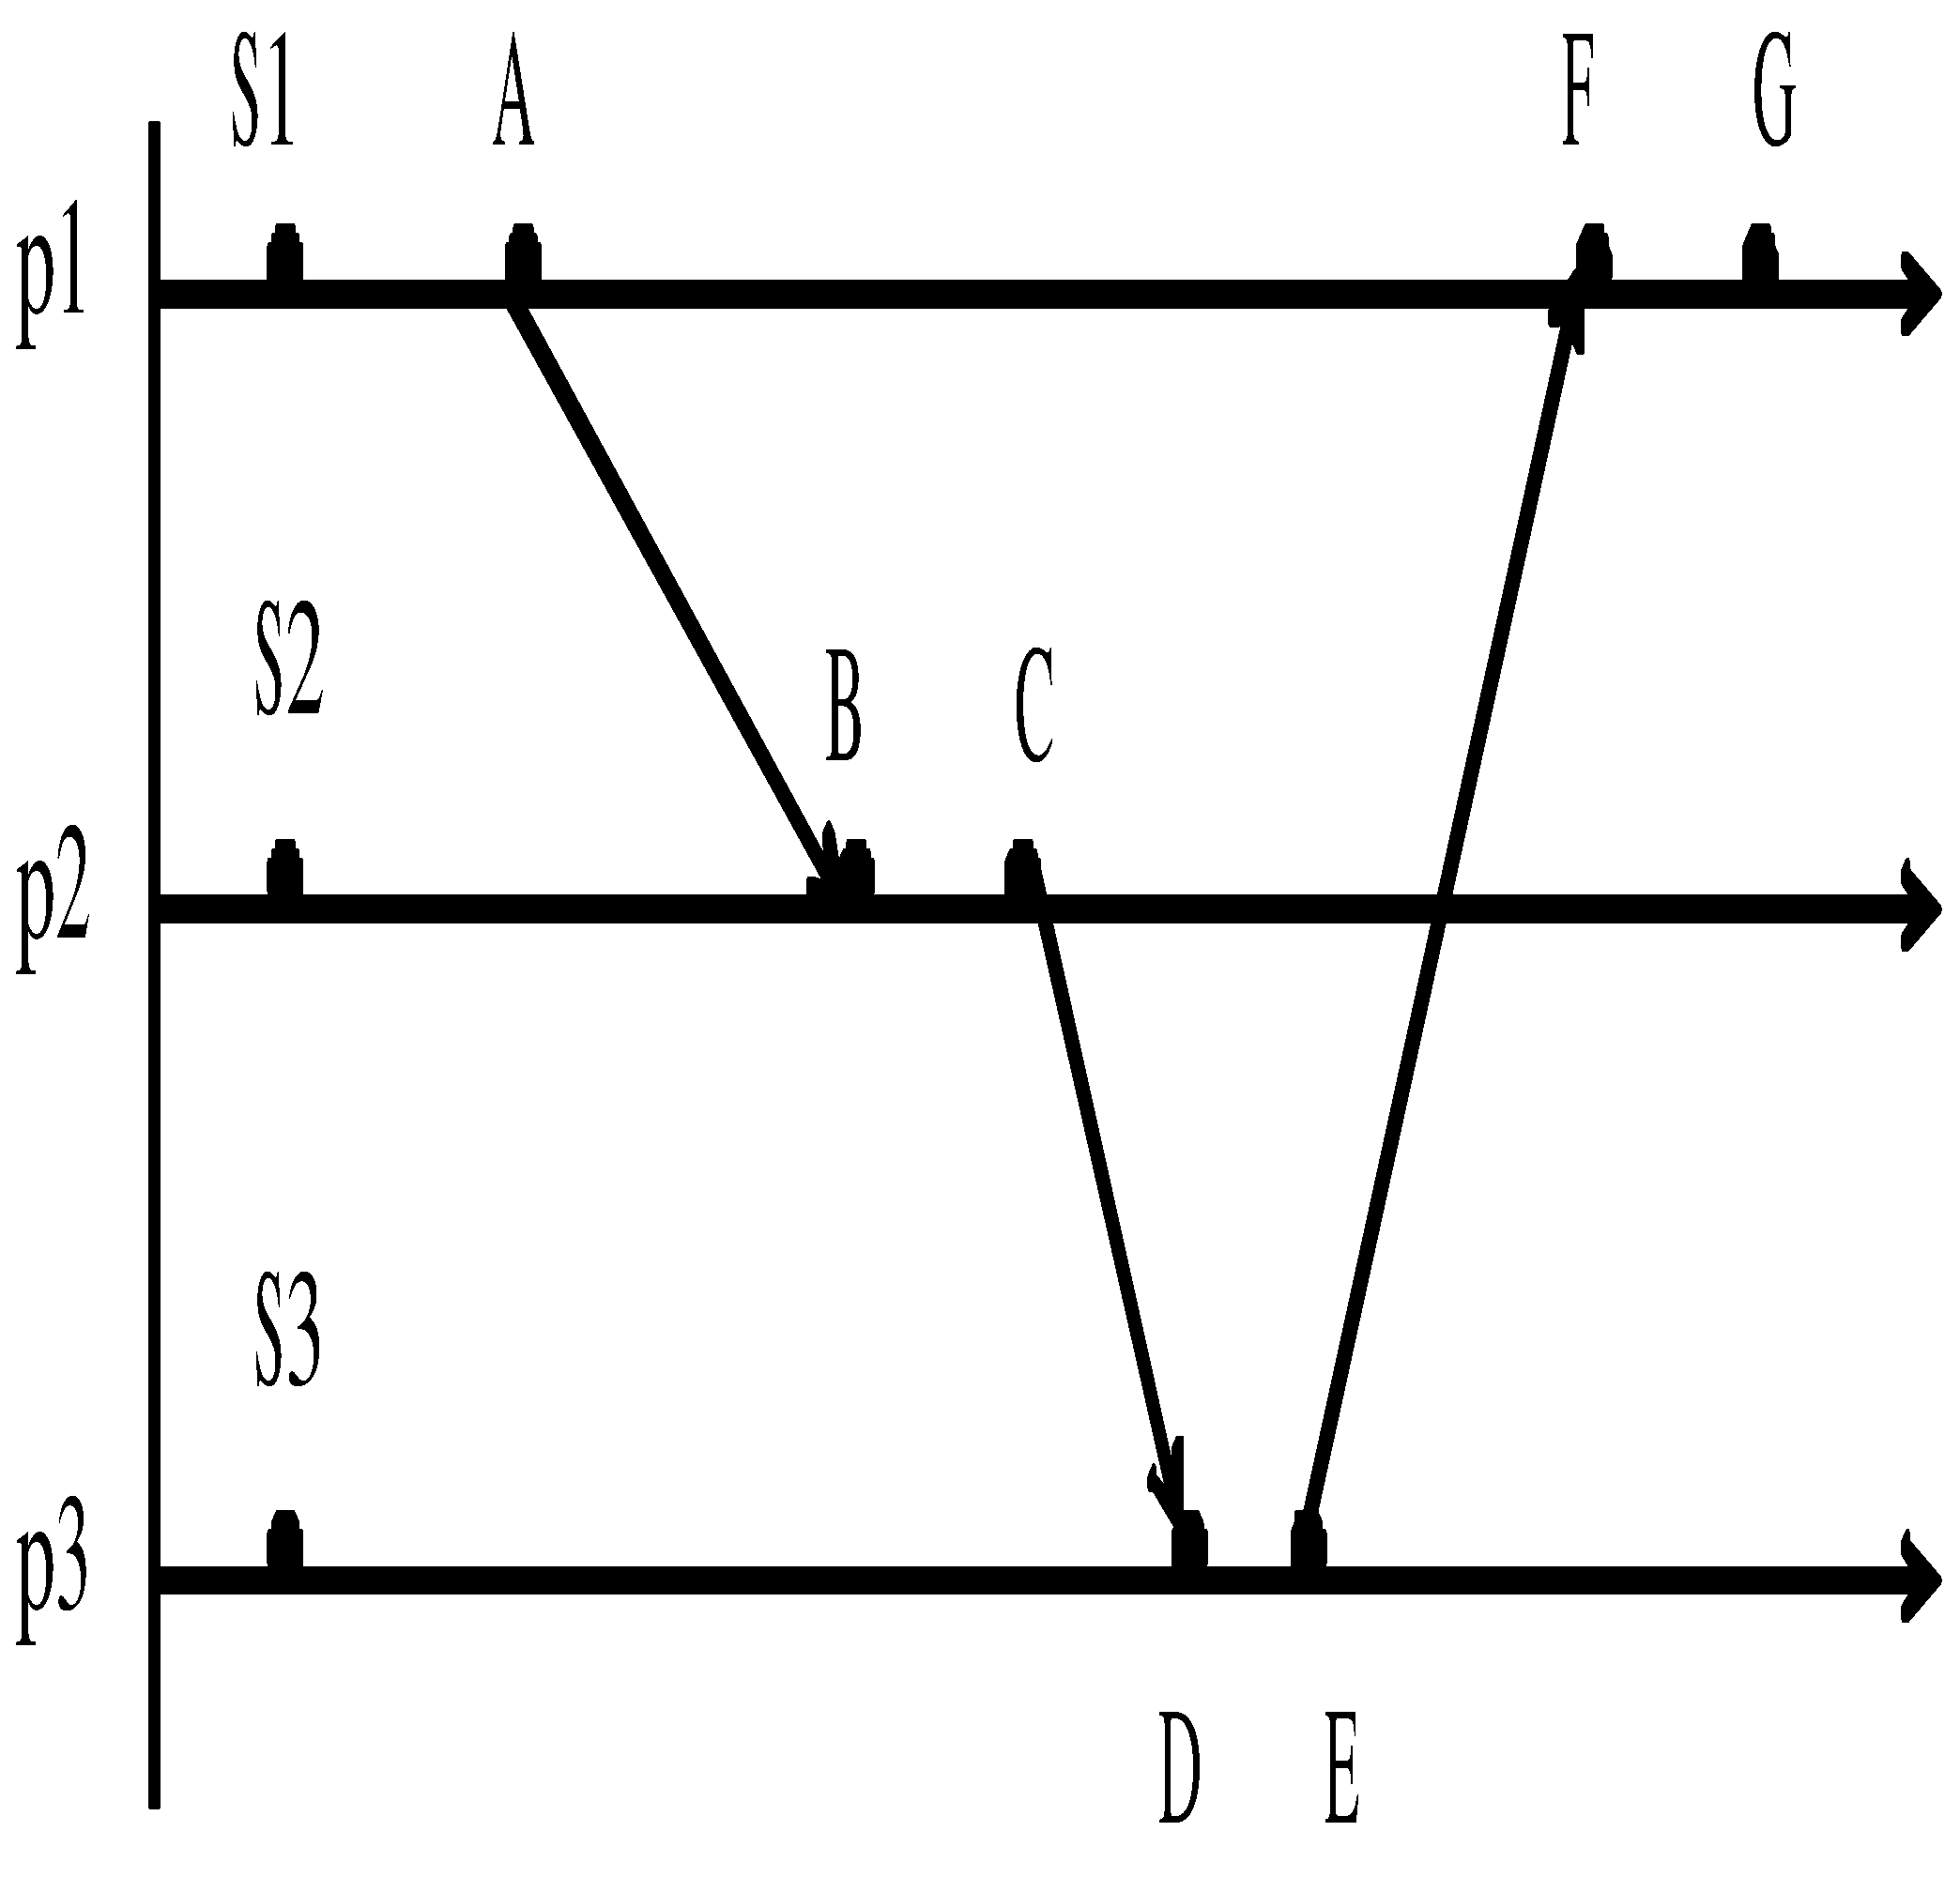
\includegraphics[height=5cm, width=7cm] {lo_logical_clock.eps}
\end{center}


    \begin{enumerate}

    \item Andrew finds out that the processes above are using Lamport's logical clock, but not all the clock values are not known to him. The initial logical time S1, S2 and S3 were 11, 1 and 0 respectively, and Andrew observed that the clock was 16 at E. What is the value of the clock at A, B, C, D, and F? \textbf{[5 points]}
    \item This time, Andrew finds out that the processes above are using vector clocks, but not all the clock values are not known. The initial logical time S1, S2 and S3 were (0,0,0) , (0,1,0) and (0,0,11) respectively. What's the clock values for A, B, C, D, E and F? \textbf{[6 points]}
    \item Give an example that highlights the shortcomings of Lamport’s clock in comparison to vector clocks, i.e., the Lamport’s algorithm cannot clearly conclude that an event e happens before $e’$, even though $L(e) < L(e’)$, where $L(e)$ is the Lamport’s timestamp of the event $e$ and that the vector clock algorithm concludes clearly whether an event $e$ happened before $e’$ or not. \textbf{[4 points]}
    
    \end{enumerate}


\item An NTP server B receives server A’s message at 11:25:12.350 bearing a timestamp 11:25:2.300 and replies to it. A receives the message at 11:25:4.620, bearing B’s timestamp 11:25:14.600. Estimate the offset between B and A and the accuracy of the estimate. \textbf{[8 points]}



    

\end{enumerate}


\end{document}
